\documentclass[12pt]{beamer}
\usepackage{amsmath,amssymb,amsfonts,amsthm}
\beamertemplatefootpagenumber
\usepackage{threeparttable}
\geometry{paperwidth=150mm,paperheight=125mm}
\usepackage{lipsum}
\usepackage{ragged2e} % 文字向兩邊對齊
\useinnertheme{rectangles}  % change the theme

\usepackage{float}
\usepackage{multirow}
\usepackage{makecell}
\usepackage{siunitx}
%\usepackage{booktabs}

%打中文需要以下packages
\usepackage{xeCJK} 
\setCJKmainfont[BoldFont={cwTeXHeiBold}, ItalicFont={FandolSong}]{cwTeXMing} %Overleaf 中文字型設定
%\setCJKmainfont[BoldFont={cwTeX Q HeiZH}, ItalicFont={新細明體}]{cwTeX Q Ming}	
\XeTeXlinebreaklocale "zh"
\XeTeXlinebreakskip = 0pt plus 1pt %這兩行一定要加,中文才能自動換行




\title[]  
{Demand System Estimation}
\subtitle[short subtitle]{Group 5}

\author{黎宏濬 \ 林孝儒 \ 張立宏 \ 許震浩}
\institute[short]{\inst{}Department of Agricultural Economics, NTU}

\date
 {October 4, 2024}
 
\AtBeginSection[]{
    % \begin{frame}[plain]  % plain 选项去除页眉页脚
    %     \vfill
    %     \figureing
    %     \usebeamerfont{section title}\insertsectionhead\par
    %     \vfill
    % \end{frame}
    \begin{frame}
        \frametitle{Outline}
        % Display the entire table of contents instead of limiting to 1-\thesection
        \tableofcontents[currentsection]
    \end{frame}
} 

\begin{document}

% Title page
\begin{frame}{}
    \titlepage
\end{frame}

% Table of Contents slide
\begin{frame}
    \frametitle{Outline}
    \tableofcontents[]
\end{frame}


\section{資料來源與資料整理過程}

\begin{frame}{資料來源}
	\begin{itemize}
		\item \textbf{經濟部 工業產銷存動態調查} 
		\begin{itemize}
			\vspace*{0.1cm}
			\item 產品價量資料(果蔬汁飲料、碳酸飲料、運動飲料、咖啡飲料、茶類飲料): 月資料, 1991年1月至2024年6月 \vspace*{0.1cm}
		\end{itemize} \vspace*{0.3cm}

		\item \textbf{勞動部 勞動統計查詢網}
		\begin{itemize}
			\vspace*{0.1cm}
			\item 國民所得統計: 月資料, 1991年1月至2024年6月
		\end{itemize} \vspace*{0.3cm}

		\item \textbf{中華民國統計資訊網 國民所得及經濟成長統計資料庫}
		\begin{itemize}
			\vspace*{0.1cm}
			\item 家庭收支統計: 年資料,1991年至2024年\vspace*{0.1cm}
			\item 物價統計(消費者物價指數、非酒精性飲料及材料物價指數): 月資料,1991年至2024年
		\end{itemize}
	\end{itemize}
\end{frame}

\begin{frame}{資料整理過程}
	\begin{itemize}
		\item \textbf{計算價格}
		\begin{itemize}
			\vspace*{0.1cm}
			\item 每月單位價格 = 每月銷售值 ÷ 每月銷售量 \vspace*{0.1cm}
			\item 名目價格需進行平減,轉換為實質價格
		\end{itemize}
		\vspace*{0.3cm}

		\item \textbf{推估月度收入}
		\begin{itemize}
			\vspace*{0.1cm}
			\item 國民所得統計:季資料 → 線性插值推估月資料 \vspace*{0.1cm}
			\item 家庭收支統計:年資料 → 線性插值推估月資料
		\end{itemize}
	\end{itemize}
\end{frame}

\begin{frame}{資料整理過程}{銷售價格的計算}
	每月的銷售價格可透過以下公式計算:
	\[
		\text{價格} = \frac{\text{每月銷售值}}{\text{每月銷售量}}
	\]
	\begin{itemize}
		\item \textbf{每月銷售值}: 表示當月的銷售總額,通常以名目貨幣計價(未調整物價變動)。\vspace*{0.1cm}
		\item \textbf{每月銷售量}: 表示當月的銷售商品數量或銷售單位。
	\end{itemize} \vspace*{0.3cm}
	透過該公式,可以估算出每月的平均銷售價格。然而,這些價格數據是名目價格,因此需要進行平減以考慮物價變動。
\end{frame}

\begin{frame}{資料整理過程}{銷售價格的計算}
	由於國民所得統計僅提供季資料,而家庭收支統計則只有年度資料,因此需要透過線性插值的方式,將這些資料轉換為月度資料,以便用於月度的需求分析。具體方法為:
	\[
		\text{收入}_m = \text{收入}_{Q1} + \left( \frac{\text{收入}_{Q2} -\text{收入}_{Q1}}{3} \right) \times (m-1)
	\]
	\begin{itemize}
		\item $m$ 表示當月的序數(1、2、3 分別對應季中的三個月)或當年的月份。 \vspace*{0.1cm}
		\item $\text{收入}_{Q1}$和$\text{收入}_{Q2}$分別表示相鄰兩個季度或年度的收入資料。
	\end{itemize} \vspace*{0.3cm}
	線性插值的假設是收入變化在兩個數據點之間是線性的,這是一種常見的簡化方法。這樣可以生成月度的收入數據,用於後續的需求分析。
\end{frame}

\begin{frame}{資料整理過程}{CPI平減價格與收入}
	\begin{itemize}
		\item \textbf{價格平減}: 由於每月計算出的銷售價格是名目價格,需要使用CPI進行平減,以得到實質價格。平減公式為:
		\[
			\text{實質價格} = \frac{\text{名目價格}}{\textrm{CPI}} \times 100
		\]
		CPI是某一年的基準值為100的價格指數,反映了物價水準的變化。實質價格能更真實地反映消費者在不同時間點上的購買力。  \vspace*{0.3cm}
		\item \textbf{收入平減}: 同樣地,收入數據也需要使用CPI進行平減,轉換為實質收入,以消除通貨膨脹的影響。平減公式為:
		\[
			\text{實質收入} = \frac{\text{名目收入}}{\textrm{CPI}} \times 100
		\]
		這樣可以得到實質的月度收入資料,用於需求系統的估計。
	\end{itemize} \vspace*{0.3cm}
\end{frame}

\section{主要變數之定義}

\begin{frame}{資料整理過程}{銷售價格的計算}
	\begin{itemize}
		\item \textbf{銷售值}:每月銷售值(單位:千元新台幣) \vspace*{0.3cm}
		\item \textbf{銷售量}:每月銷售量(單位:千公升)\vspace*{0.3cm}
		\item \textbf{單位價格}:每月銷售商品之單位價格(單位:千元新台幣/千公升)\vspace*{0.3cm}
		\item \textbf{國民所得}:平均每人薪資所得月資料(單位:元新台幣)\vspace*{0.3cm}
		\item \textbf{家庭收支}:平均每戶薪資所得月資料(單位:元新台幣)
	\end{itemize}
\end{frame}

\section{主要變數之敘述統計}

\begin{frame}{主要變數之敘述統計}{銷售值}
	\begin{figure}
		\centering
		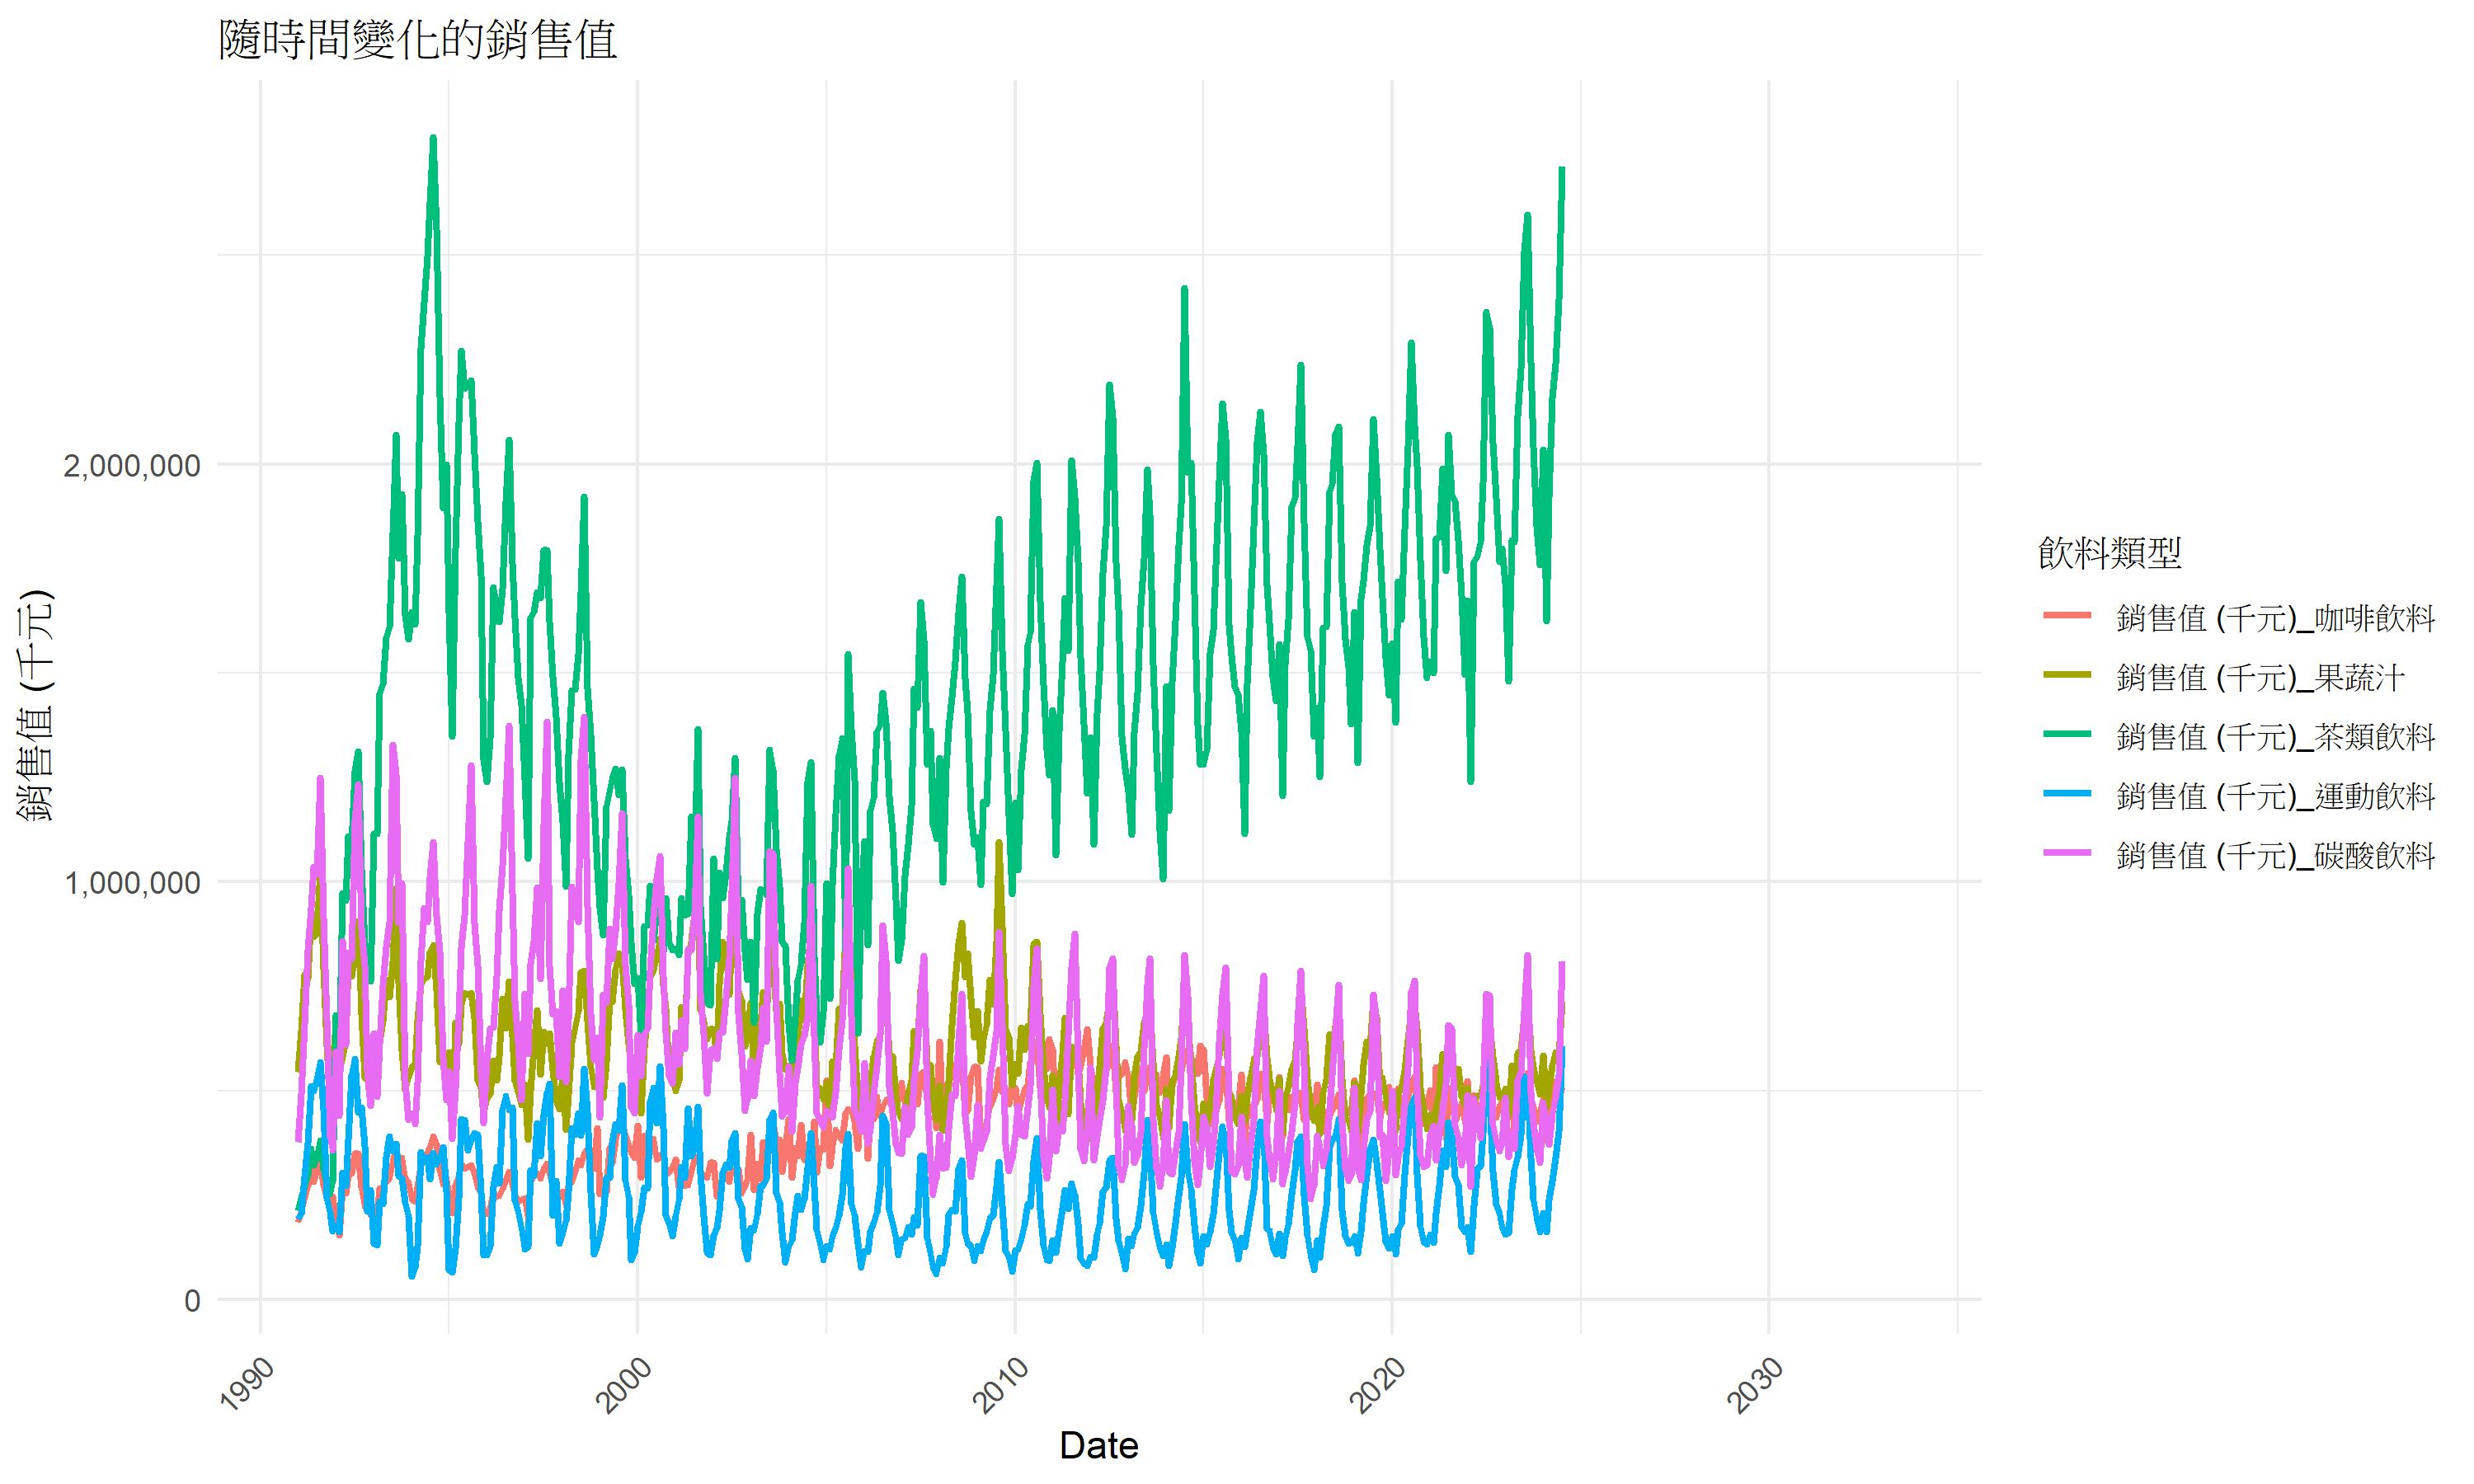
\includegraphics[width=0.7\textwidth]{figures/銷售值.jpg}
		\caption{各項商品歷年銷售值}
	\end{figure}
	% \begin{itemize}
	% 	\item 
	% \end{itemize}
\end{frame}

\begin{frame}{主要變數之敘述統計}{銷售值}
	\begin{center}
	 \begin{tabular}{ c r r r r r} 
	  \hline
	  & \multicolumn{5}{c}{銷售值(千元新台幣)} \\
	  & 果蔬汁 & 碳酸飲料 & 運動飲料 & 咖啡飲料 & 茶類飲料 \\ 
	  \hline
	  mean & 602385 & 586043 & 248529 & 410575 & 1434599 \\ 
	  sd & 133688 & 241157 & 121843 & 107838 & 480714 \\
	  median & 580869 & 522322 & 217915 & 429376 & 1452576 \\ 
	  min & 338694 & 241473 & 54881 & 153917 & 213117  \\ 
	  max & 1096399 & 1394424 & 606710 & 647208 & 2781819 \\ 
	  range & 757705 & 1152951 & 551829 & 493291 & 2568702 \\ 
	  n & \multicolumn{5}{c}{403} \\
	  \hline
	 \end{tabular}
	\end{center}
\end{frame}

\begin{frame}{主要變數之敘述統計}{銷售量}
	\begin{figure}
		 
  		\centering
		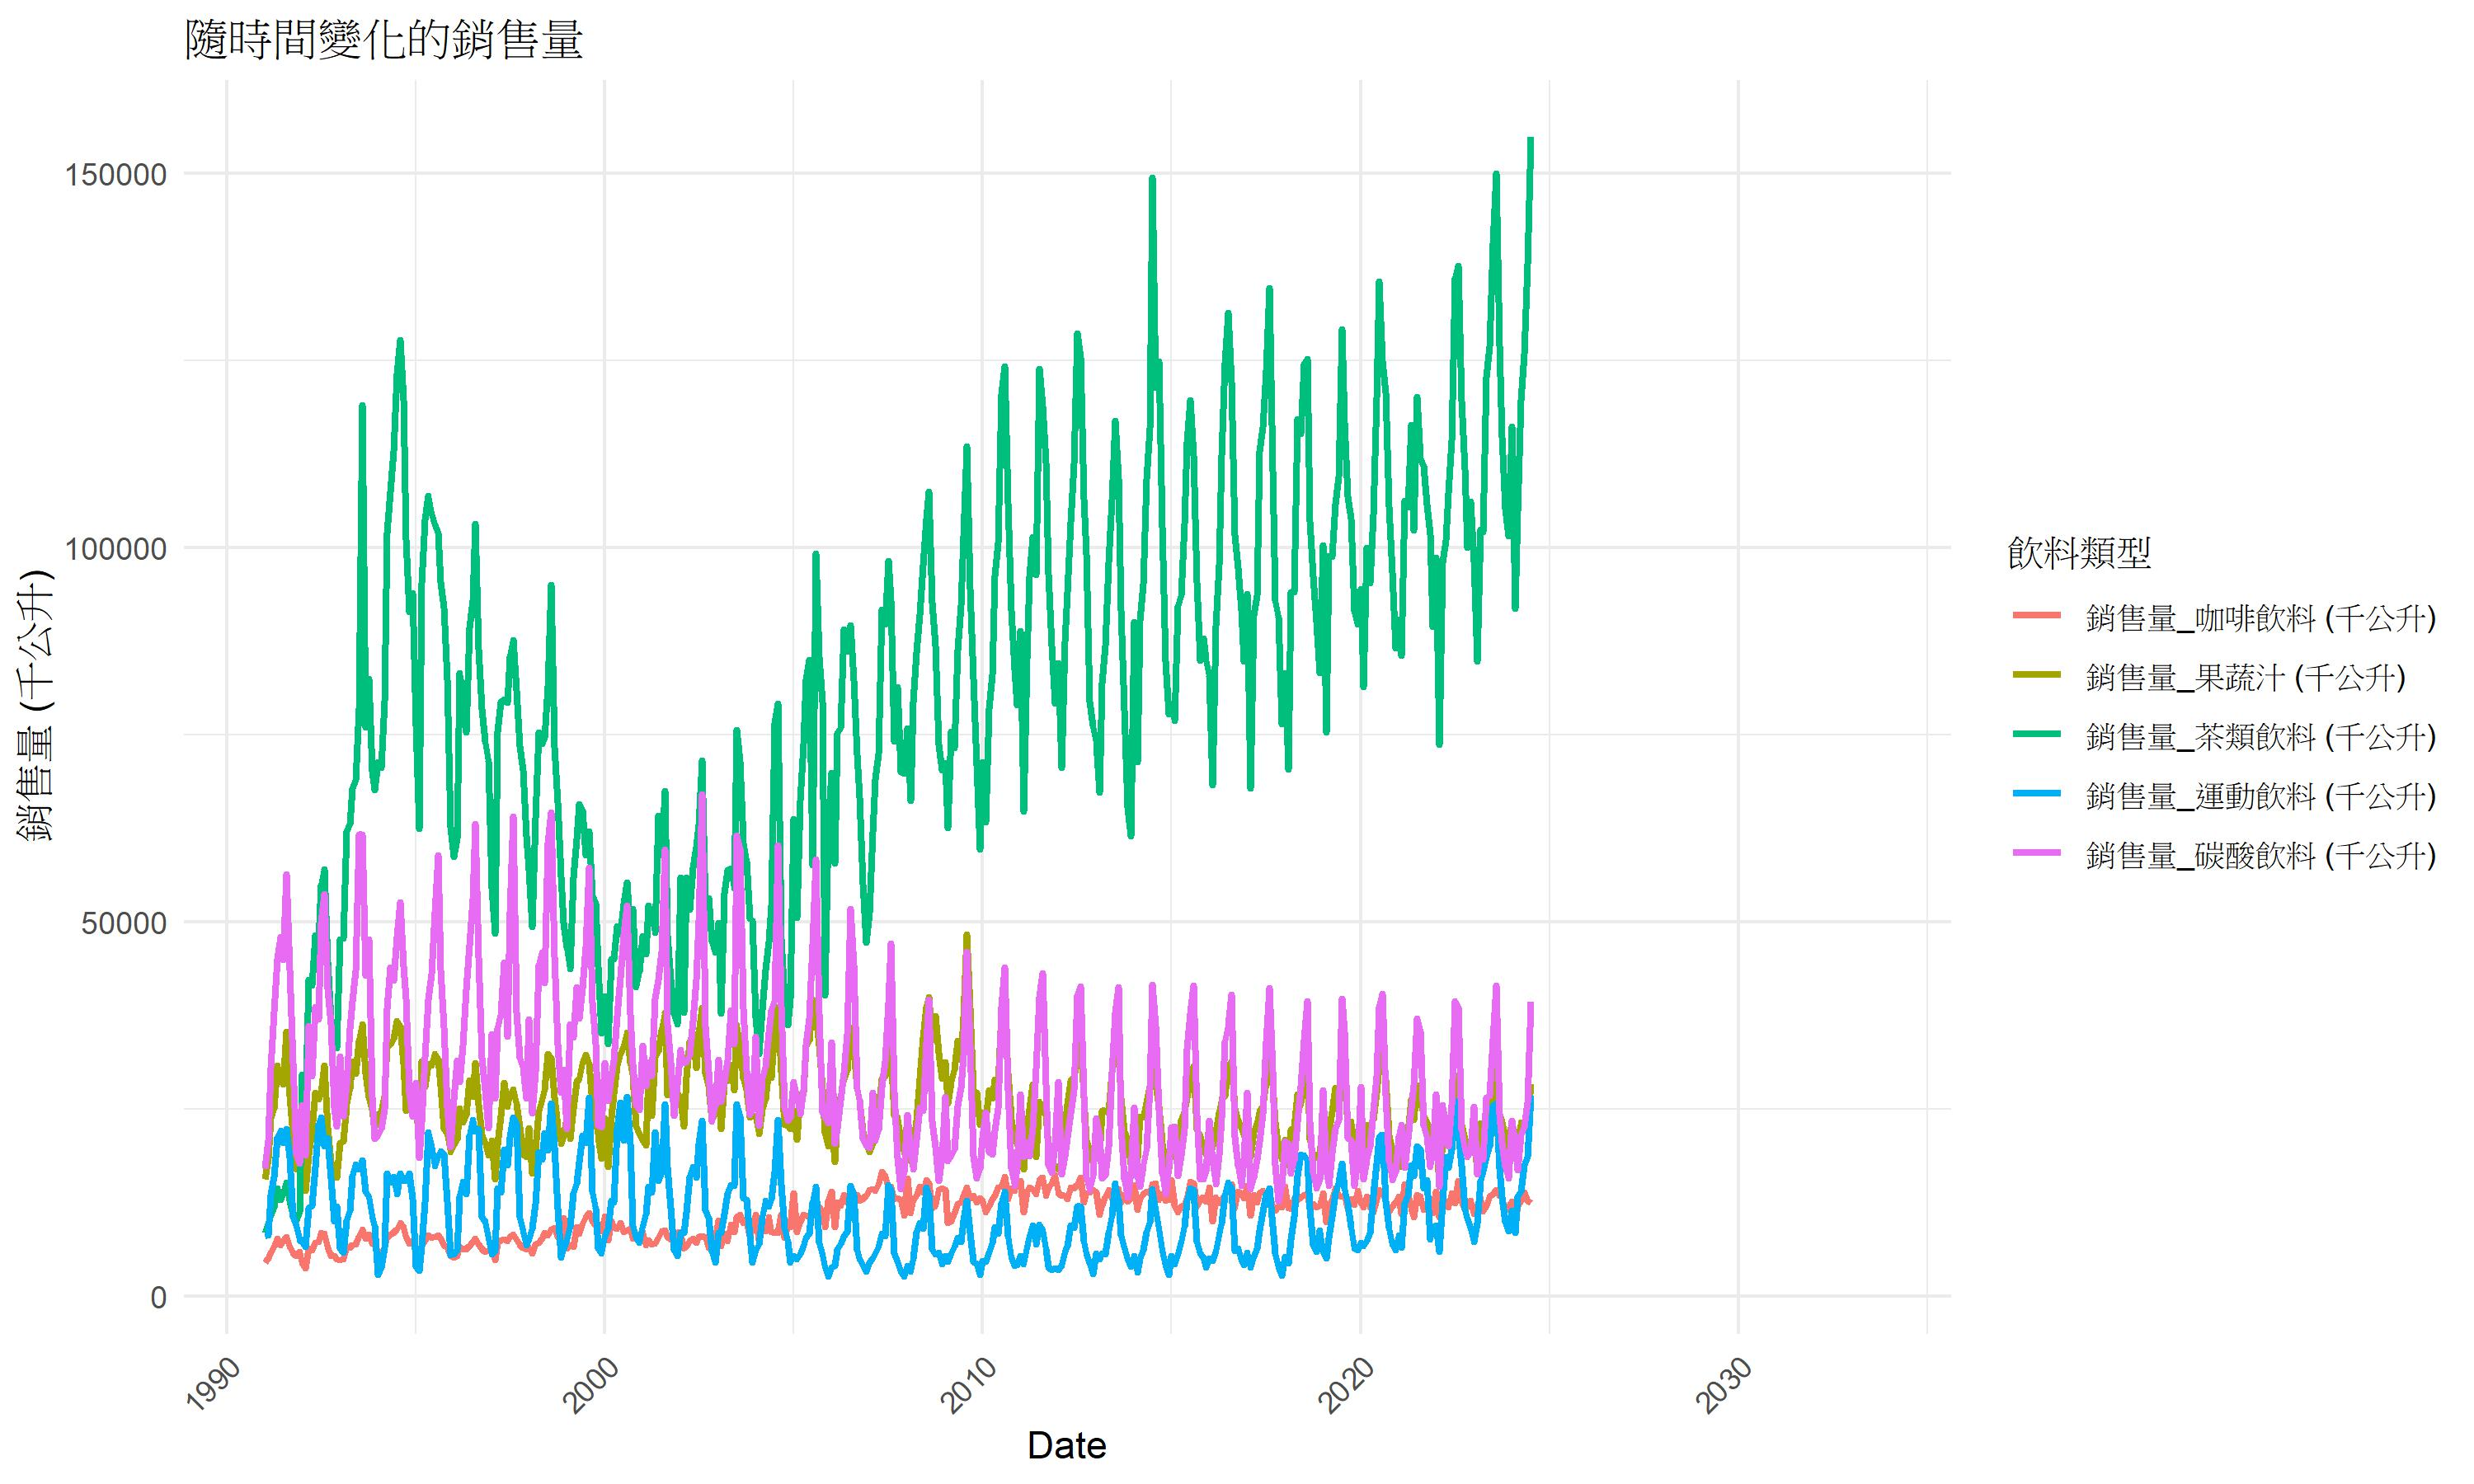
\includegraphics[width=0.7\textwidth]{figures/銷售量.jpg}
		\caption{各項商品歷年銷售量}
	\end{figure}
	% \begin{itemize}
	% 	\item 
	% \end{itemize}
\end{frame}

\begin{frame}{主要變數之敘述統計}{銷售量}
	\begin{center}
	 \begin{tabular}{ c r r r r r} 
	  \hline
	  & \multicolumn{5}{c}{銷售量(千公升)} \\
	  & 果蔬汁 & 碳酸飲料 & 運動飲料 & 咖啡飲料 & 茶類飲料 \\ 
	  \hline
	  mean & 25567 & 29496 & 11152 & 10801 & 80623 \\ 
	  sd & 5453 & 11374 & 5934 & 3044 & 28261 \\
	  median & 24768 & 26785 & 9489 & 11584 & 82310 \\ 
	  min & 14158 & 12690 & 2614 & 3714 & 8525  \\ 
	  max & 48324 & 67064 & 26808 & 16673 & 154863 \\ 
	  range & 34166 & 54374 & 24194 & 12959 & 146338 \\ 
	  n & \multicolumn{5}{c}{403} \\
	  \hline
	 \end{tabular}
	\end{center}
\end{frame}

\begin{frame}{主要變數之敘述統計}{單位價格}
	\begin{figure}
 		\centering
		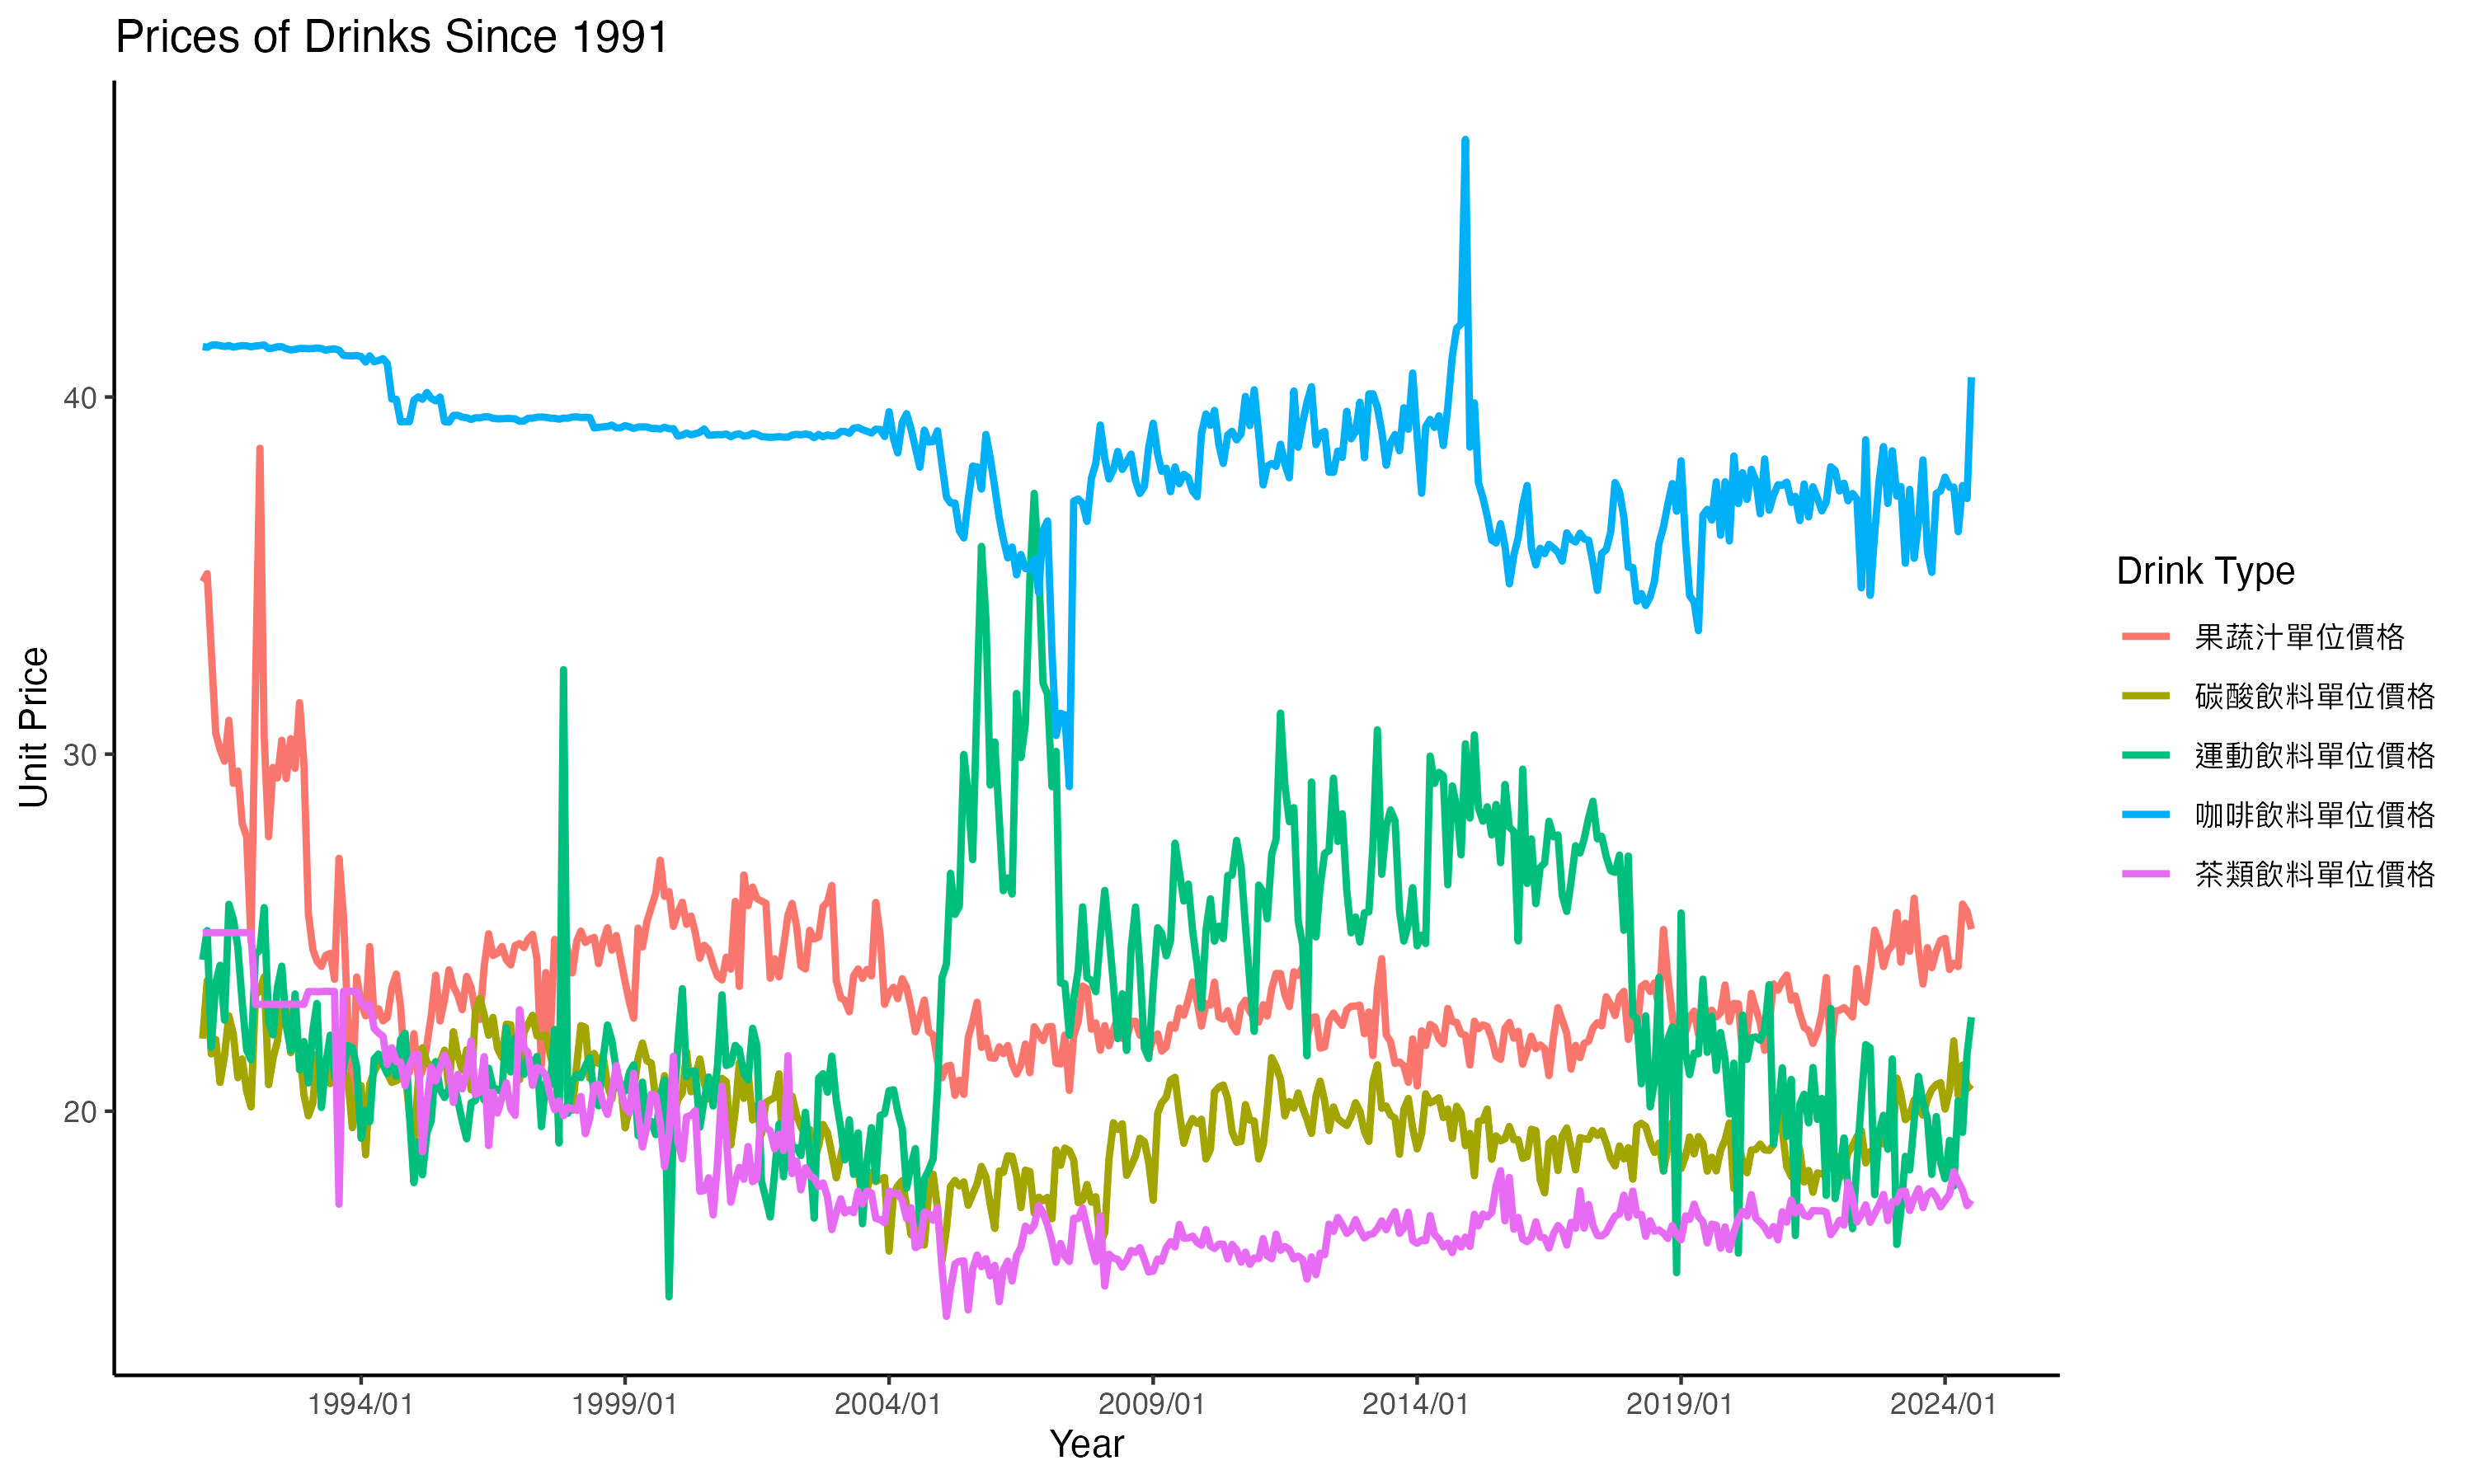
\includegraphics[width=0.7\textwidth]{figures/drinks_prices_plot.jpg}
		\caption{各項商品歷年單位價格}
	\end{figure}
	% \begin{itemize}
	% 	\item 
	% \end{itemize}
\end{frame}

\begin{frame}{主要變數之敘述統計}{國民所得}
	\begin{figure}
		 
  		\centering
		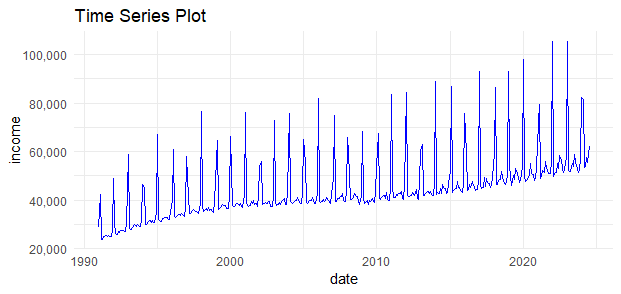
\includegraphics[width=0.7\textwidth]{figures/國民所得.png}
		\caption{歷年國民所得}
	\end{figure}
	% \begin{itemize}
	% 	\item 
	% \end{itemize}
\end{frame}

\begin{frame}{主要變數之敘述統計}{家庭收支}
	\begin{figure}
		 
 		\centering
		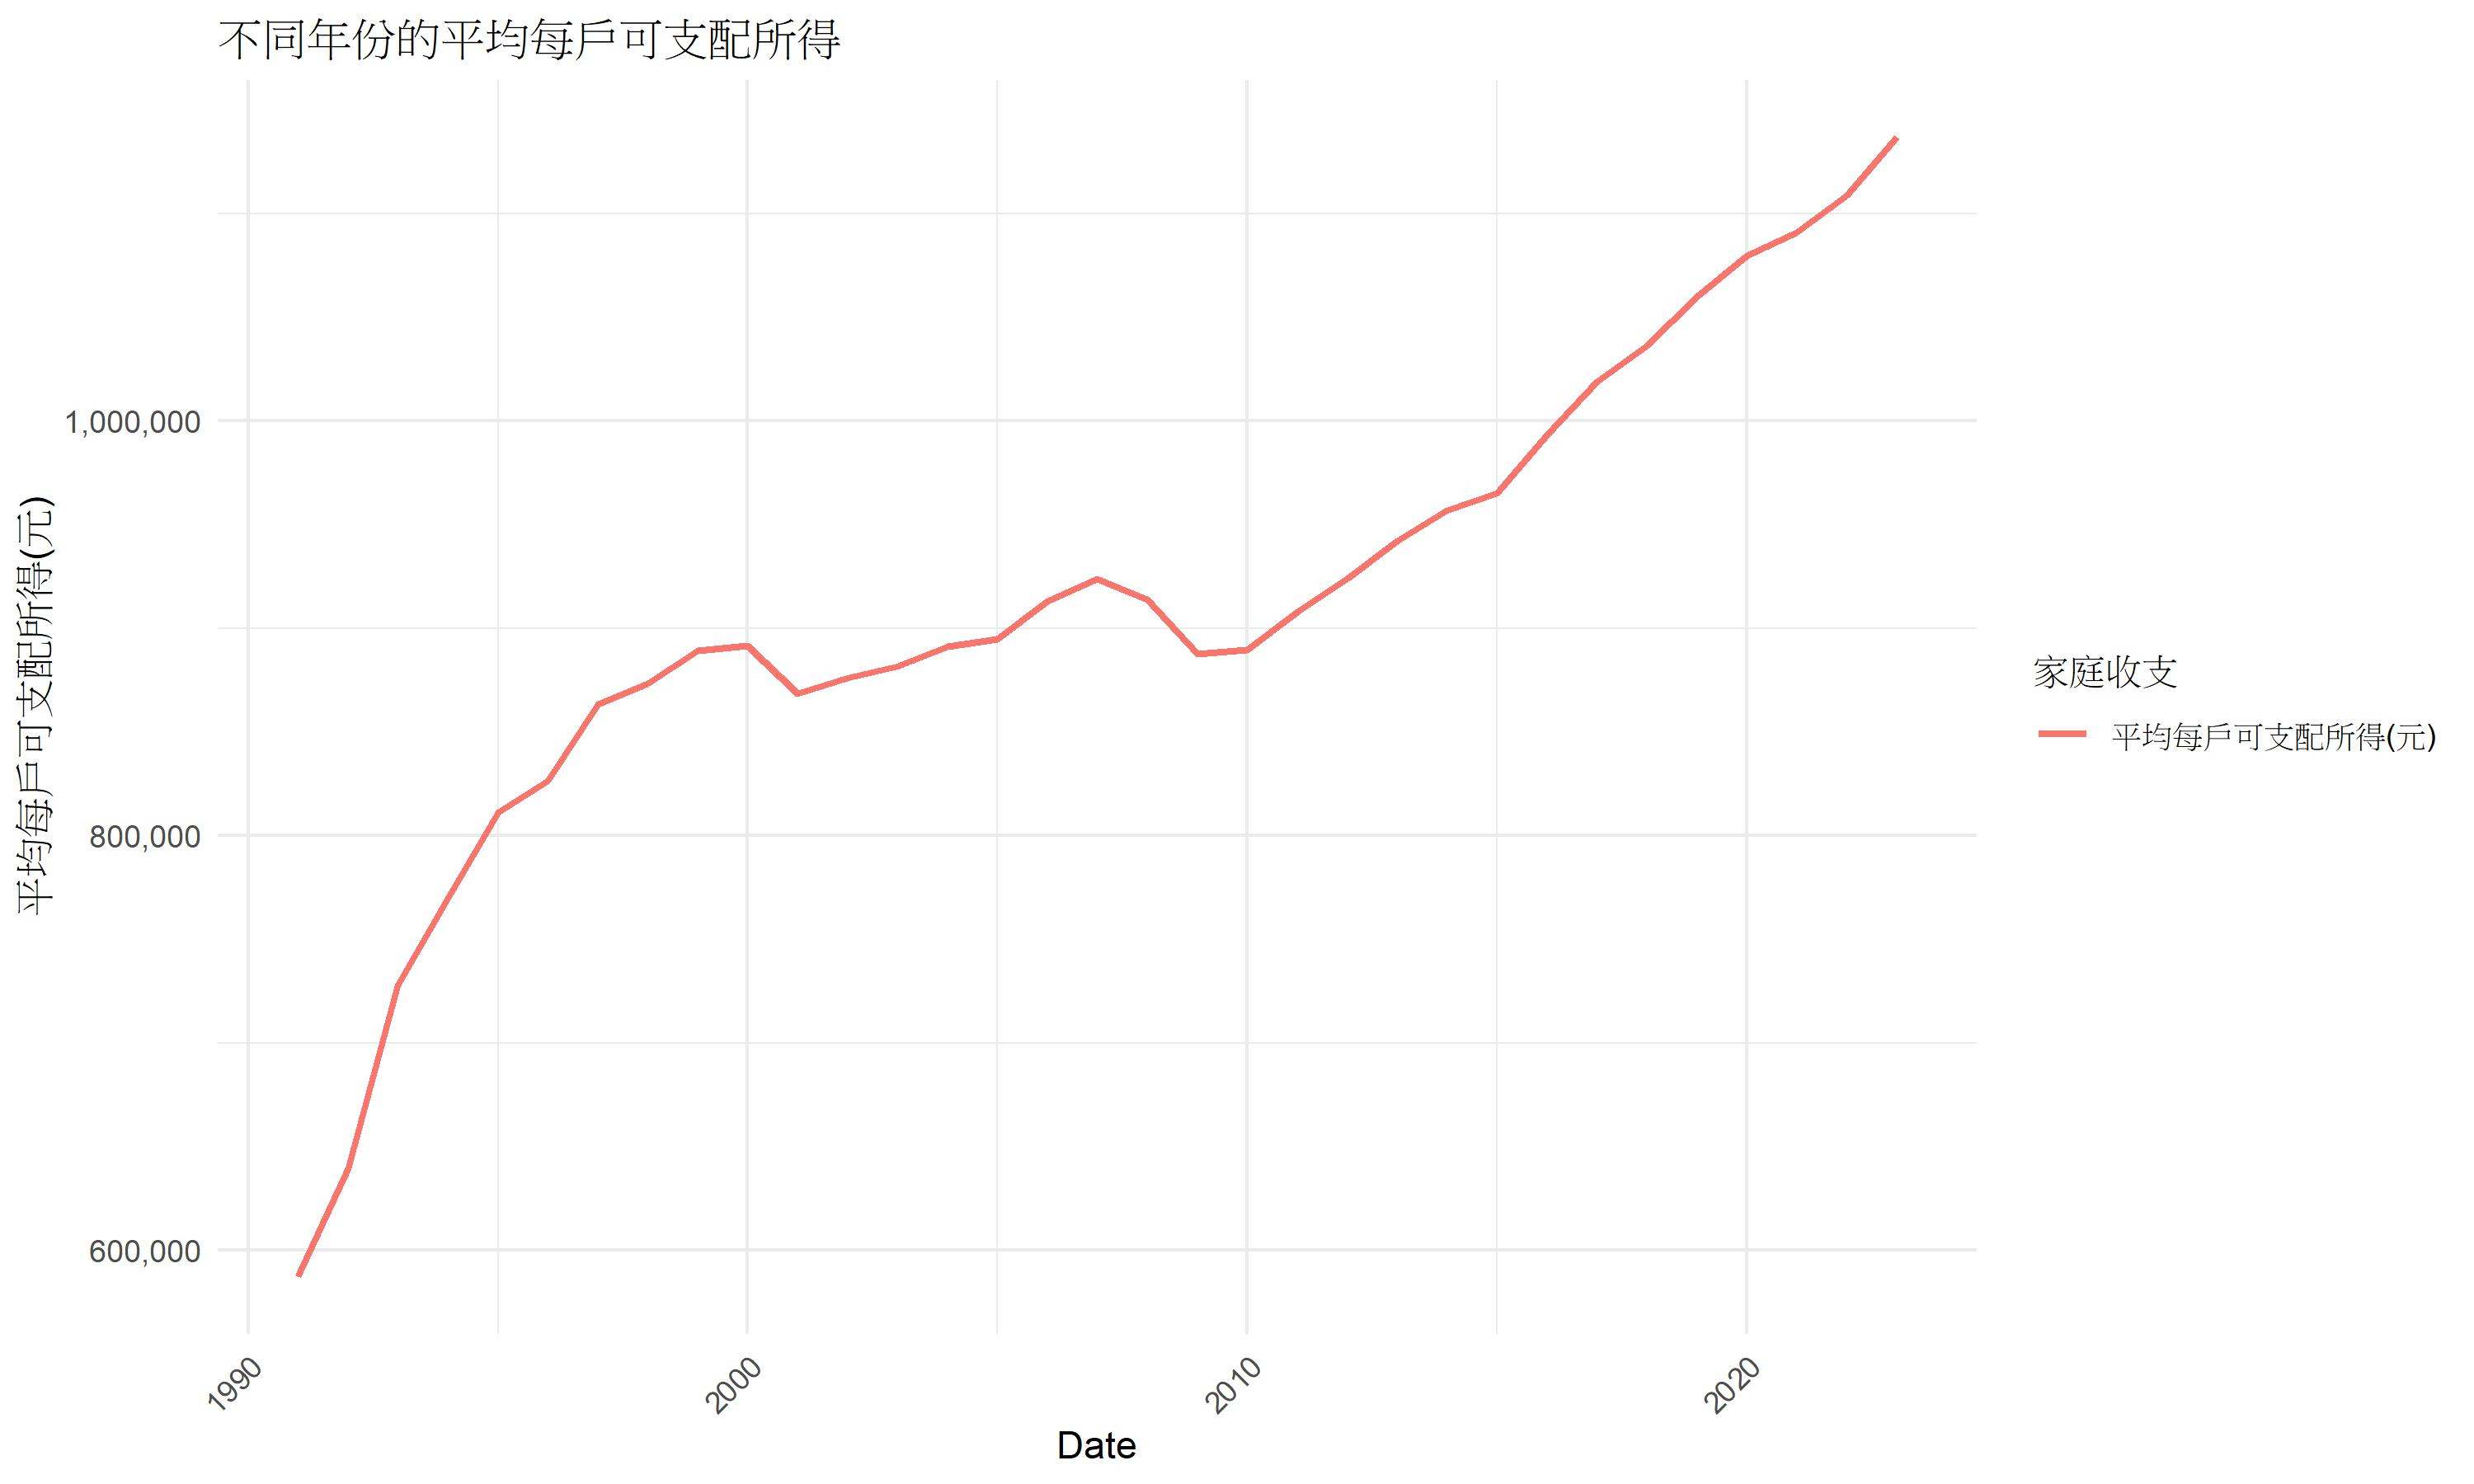
\includegraphics[width=0.7\textwidth]{figures/家庭收支.jpg}
		\caption{歷年家庭收支}
	\end{figure}
	% \begin{itemize}
	% 	\item 
	% \end{itemize}
\end{frame}

\begin{frame}{主要變數之敘述統計}{}
	\begin{center}
	 \begin{tabular}{ c r r} 
	  \hline
	  & 國民所得(元新台幣) & 家庭收支(元新台幣) \\ 
	  \hline
	  mean & 44379 & 910246  \\ 
	  sd & 12770 & 121488  \\
	  median & 41565 & 894574  \\ 
	  min & 23829 & 587242  \\ 
	  max & 105379 & 1136708  \\ 
	  range & 81550 & 549466 \\ 
	  n & \multicolumn{2}{c}{403} \\
	  \hline
	 \end{tabular}
	\end{center}
\end{frame}

% \begin{frame}{Q3: What products are you going to choose to form a demand system and why (the significance of your study)?}
% 	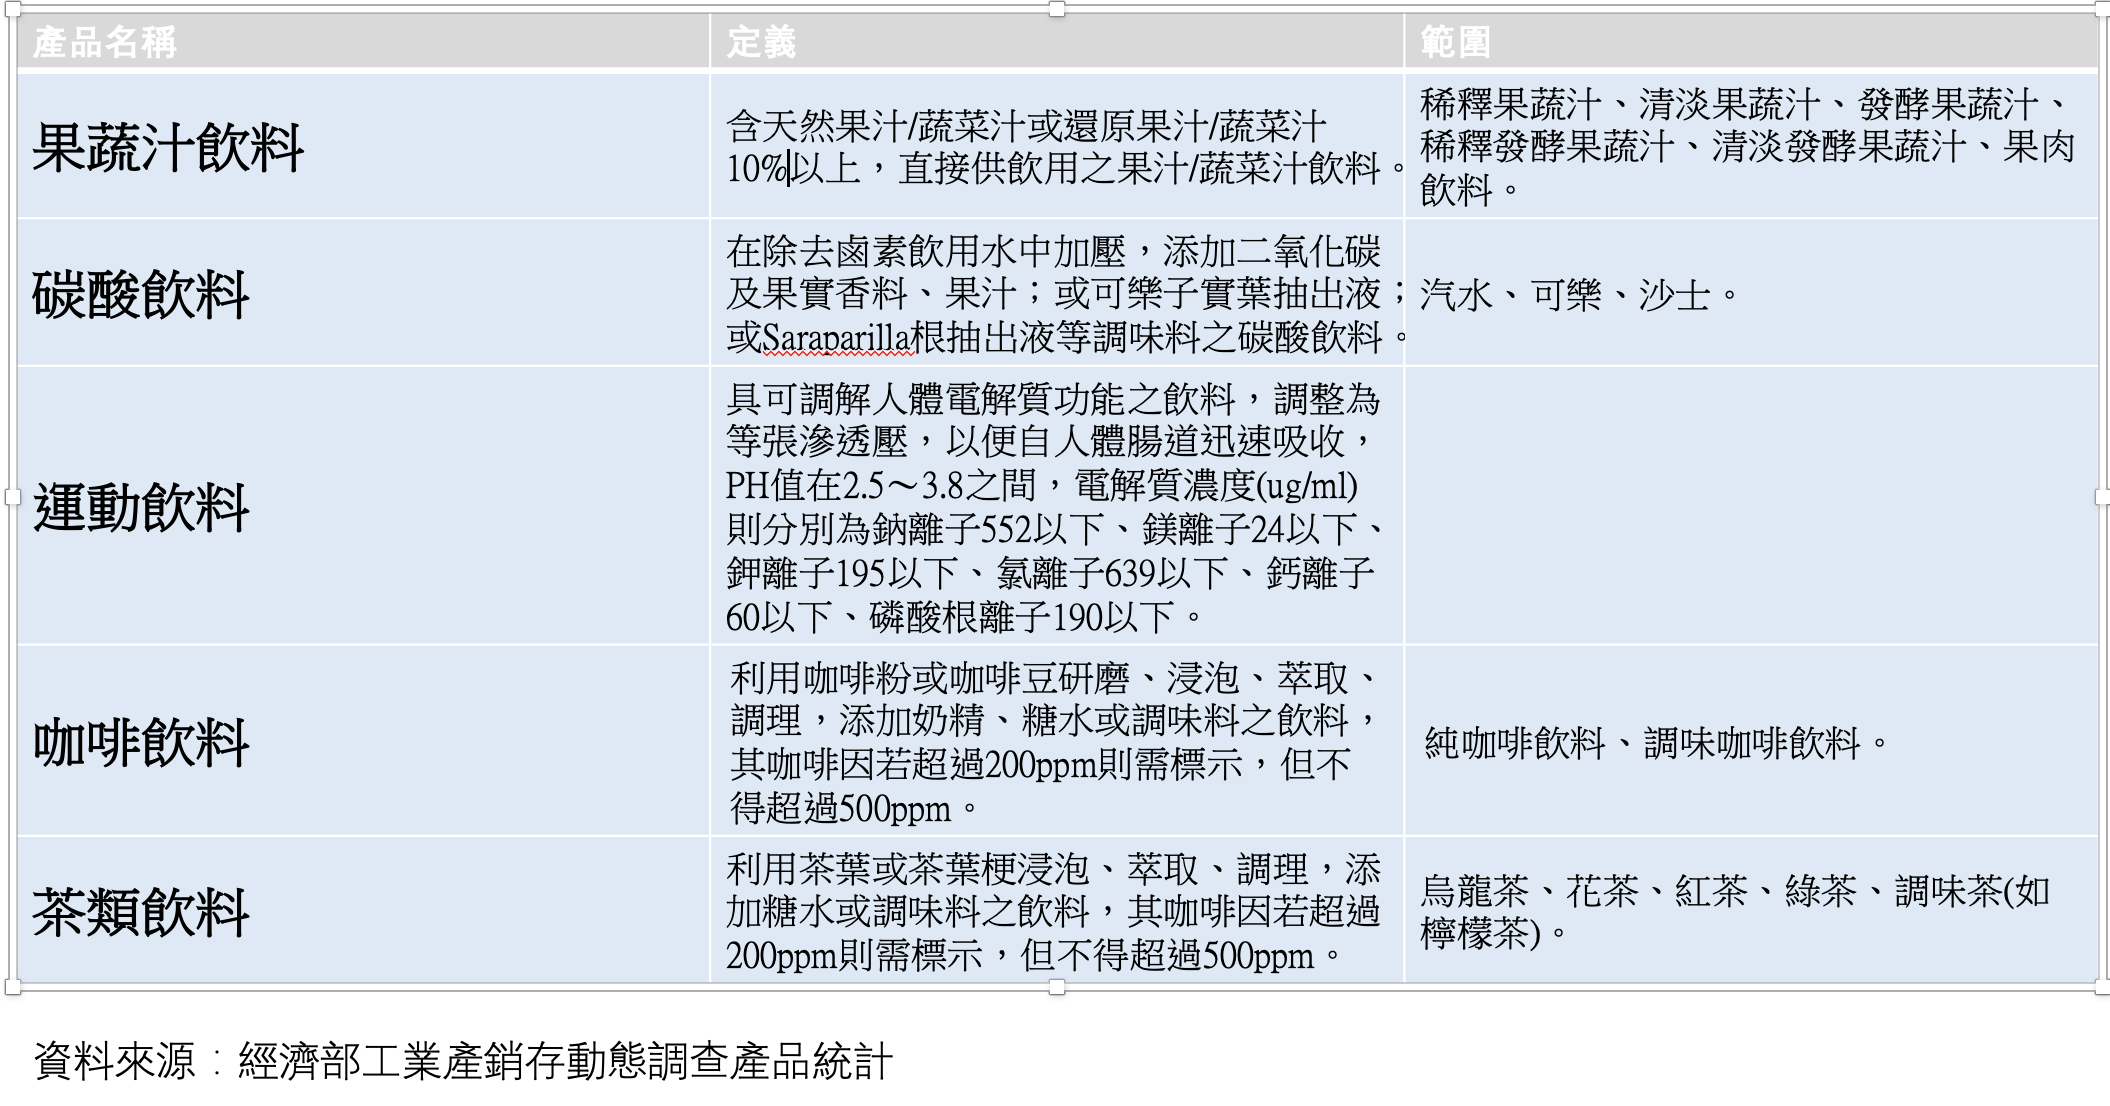
\includegraphics[width=0.7\textwidth]{figures/fig.png}
% \end{frame}


% \begin{frame}{Q4: What are the research questions raised in your DSE?}
% 	\begin{itemize}
% 		\item \textbf{消費者對不同飲料類別的價格彈性}:當價格變動時,消費者對果蔬汁飲料、碳酸飲料、運動飲料、咖啡飲料和茶類飲料的需求如何變化?是否某一類飲品對價格更敏感?
% 		\vspace{0.3cm}
% 		\item \textbf{不同飲料類別之間的交叉價格彈性}:當一類飲品的價格上升或下降時,是否會影響其他類似飲品的需求?
% 		\vspace{0.3cm}
% 		\item \textbf{收入水準變化對消費者飲料需求的影響}:隨著消費者收入的增長或減少,哪一類飲品的需求會受到最大影響?運動飲料、果蔬汁飲料或咖啡飲料是否更依賴於收入的變化?
% 	\end{itemize}
% \end{frame}

% \begin{frame}{Q5: Please provide sufficient background information about the topic you chose for your analyses.}
% 	\begin{itemize}
% 		\item \textbf{產品的市場覆蓋率和多樣性}:五類飲料涵蓋了當今飲料市場中最重要的細分市場,能夠代表大部分消費者的飲料需求,適合進行整體飲料市場的需求體系分析。
% 		\vspace{0.3cm}
% 		\item \textbf{消費行為差異}:些飲料類型反映了不同消費需求和偏好。例如,運動飲料主要消費於運動後恢復能量,而咖啡飲料更多與提神和日常工作需求相關。年輕人可能更偏好碳酸飲料和運動飲料,而中老年人則傾向於選擇果蔬汁和茶飲。
% 		\vspace{0.3cm}
% 		\item \textbf{健康意識的影響}:隨著健康意識的提升,果蔬汁和茶飲料逐漸受到追捧,而碳酸飲料面臨健康風險相關的負面影響。在 demand system 中加入這些不同健康屬性的飲料,可以更好地分析消費者健康意識對飲料選擇的影響。
% 		\vspace{0.3cm}
% 		\item \textbf{替代效應研究}:這五種類型的飲料之間存在替代關係,通過 demand system,可以分析不同飲料類型之間的影響,從而提供更全面的消費者市場需求預測。
% 	\end{itemize}
% \end{frame}


\end{document}
